% Options for packages loaded elsewhere
\PassOptionsToPackage{unicode}{hyperref}
\PassOptionsToPackage{hyphens}{url}
%
\documentclass[
  12,
  table]{proadi}
\usepackage{lmodern}
\usepackage{amssymb,amsmath}
\usepackage{ifxetex,ifluatex}
\ifnum 0\ifxetex 1\fi\ifluatex 1\fi=0 % if pdftex
  \usepackage[T1]{fontenc}
  \usepackage[utf8]{inputenc}
  \usepackage{textcomp} % provide euro and other symbols
\else % if luatex or xetex
  \usepackage{unicode-math}
  \defaultfontfeatures{Scale=MatchLowercase}
  \defaultfontfeatures[\rmfamily]{Ligatures=TeX,Scale=1}
\fi
% Use upquote if available, for straight quotes in verbatim environments
\IfFileExists{upquote.sty}{\usepackage{upquote}}{}
\IfFileExists{microtype.sty}{% use microtype if available
  \usepackage[]{microtype}
  \UseMicrotypeSet[protrusion]{basicmath} % disable protrusion for tt fonts
}{}
\makeatletter
\@ifundefined{KOMAClassName}{% if non-KOMA class
  \IfFileExists{parskip.sty}{%
    \usepackage{parskip}
  }{% else
    \setlength{\parindent}{0pt}
    \setlength{\parskip}{6pt plus 2pt minus 1pt}}
}{% if KOMA class
  \KOMAoptions{parskip=half}}
\makeatother
\usepackage{xcolor}
\IfFileExists{xurl.sty}{\usepackage{xurl}}{} % add URL line breaks if available
\IfFileExists{bookmark.sty}{\usepackage{bookmark}}{\usepackage{hyperref}}
\hypersetup{
  hidelinks,
  pdfcreator={LaTeX via pandoc}}
\urlstyle{same} % disable monospaced font for URLs
\usepackage{graphicx,grffile}
\makeatletter
\def\maxwidth{\ifdim\Gin@nat@width>\linewidth\linewidth\else\Gin@nat@width\fi}
\def\maxheight{\ifdim\Gin@nat@height>\textheight\textheight\else\Gin@nat@height\fi}
\makeatother
% Scale images if necessary, so that they will not overflow the page
% margins by default, and it is still possible to overwrite the defaults
% using explicit options in \includegraphics[width, height, ...]{}
\setkeys{Gin}{width=\maxwidth,height=\maxheight,keepaspectratio}
% Set default figure placement to htbp
\makeatletter
\def\fps@figure{htbp}
\makeatother
\setlength{\emergencystretch}{3em} % prevent overfull lines
\providecommand{\tightlist}{%
  \setlength{\itemsep}{0pt}\setlength{\parskip}{0pt}}
\setcounter{secnumdepth}{5}
\base{aih}
\usepackage[utf8]{inputenc}
\usepackage[brazil]{babel}
\usepackage{longtable,booktabs}
\usepackage{pdflscape}
\usepackage{caption}
\usepackage{lscape}
\usepackage{xcolor}
\hypersetup{draft}

\author{}
\date{\vspace{-2.5em}}

\begin{document}

\hypertarget{qualidade-de-dados}{%
\section{Qualidade de dados}\label{qualidade-de-dados}}

O processo de análise de qualidade de dados está focado na avaliação de
conjuntos de dados e na aplicação de ações corretivas, para garantir que
estes estejam adequados aos propósitos para os quais foram originalmente
destinados (Merino et al. 2016). Dessa forma, a qualidade de dados está
diretamente relacionada a confiabilidade dos dados de entrada.
Considerando que os dados têm níveis inadequados de qualidade, é
provável que ocorram erros, que podem se propagar acidentalmente e
inconscientemente por todo o fluxo da informação, prejudicando a
eficiência do sistema. Formas regulares de avaliar a qualidade de dados
com modelos clássicos geralmente se destinam a detectar e corrigir erros
em fontes conhecidas com base em um conjunto limitado de regras. No
ambiente de \emph{Big Data}, a quantidade de regras pode ser enorme e o
custo da aplicação para correção de erros pode não ser viável e nem
apropriado. Isso ocorre principalmente porque o \emph{Big Data} não é
apenas sobre dados, mas também sobre uma pilha conceitual e tecnológica
completa, incluindo dados brutos e processados, armazenamento, formas de
gerenciar dados, processamento e análise (Merino et al. 2016).

Uma dimensão de qualidade de dados é um termo descritor de um recurso de
dados, o qual pode ser medido ou avaliado de acordo com padrões
definidos, a fim de determinar a qualidade de um conjunto de dados.
Geralmente, dados só têm valor quando dão suporte a um processo ou a uma
tomada de decisão. Em consequência, as regras de qualidade de dados
definidas devem levar em consideração o valor que os dados podem
fornecer para o sistema. Nesse contexto, as seguintes dimensões de
qualidade de dados são analisadas: Completude, Conformidade, Acurácia,
Consistência, Unicidade, Temporalidade

\textbf{Completude} caracteriza a taxa de preenchimento das variáveis.
Para cada variável é calculado o percentual de entradas com informação
não nulas, respeitando, quando houver, sua dependência com outras
variáveis.

\textbf{Conformidade} detecta concordância nos valores digitados nos
campos das variáveis, avaliando se os valores de entrada não nulos estão
em conformidade com os padrões descritos pelo dicionário de dados. Para
cada variável estudada é calculado o percentual de entradas em
conformidade com o padrão adotado.

\textbf{Acurácia} visa detectar se informação registrada reflete o
evento ou objeto descrito, isto é, verificar se o dado cadastrado está
em concordância com o evento observado. Devido ao processo de
anonimização dos dados, a análise de acurácia se restringe a verificar a
possibilidade das informações registradas. Note que acurácia e
conformidade são dimensões distintas, pois enquanto conformidade avalia
o padrão do dado, acurácia avalia a razoabilidade dos dados. Para cada
variável estudada é calculado o percentual de entradas com informações
acuradas.

\textbf{Consistência} constitui de testes envolvendo duas ou mais
variáveis visando detectar inconsistências entre dados de um mesmo
registro. Para cada teste considerado é calculado os percentuais de
aprovação e falha.

\textbf{Unicidade} objetiva mensurar o grau de duplicidade nos dados,
realizando a busca por meio de identificadores dos pacientes.

\textbf{Temporalidade} objetiva efetuar medidas estatísticas nos
intervalos de tempos entre eventos, por exemplo, o nascimento de um
recém-nascido e inclusão desse registro no sistema. O principal
interesse é verificar se o dado é disponibilizado prontamente.

\renewcommand{\arraystretch}{1.25}

\renewcommand{\arraystretch}{1}

\hypertarget{muxe9todos}{%
\section{Métodos}\label{muxe9todos}}

A análise apresentada constitui-se de um esquema cíclico, iniciando no
mapeamento da documentação e do comportamento dos dados, através da
observação de trechos das bases. Em seguida, são definidas as variáveis
de teste. Após, ocorre a obtenção e avaliação dos resultados obtidos,
recorrendo, e se necessário retificando, conclusões obtidas nos passos
anteriores. Nesse contexto, são definidos parâmetros a serem passados
para as funções relativas às metricas citadas e implementação de
\emph{queries} para os testes de consistência, sintetizados em um único
\emph{script} relativo à base analisada.

O maneio dos dados ocorreu através dos serviços \textbf{Amazon Athena} e
\textbf{Amazon S3}, assim como testes e análises se deu utilizando
\textbf{linguagem R}. Os \emph{scripts} utilizados estão disponíveis em
um repositório de qualidade de dados no \emph{GitHub}. Enfatiza-se que
esses dados podem sofrer alterações, caso ocorram atualizações.

O dicionário de dado utilizado, não oficial, é inferido das descrições
das variáveis contidas nos relatórios de integração e é apresentado
neste relatório. No que tange os testes de unicidade, procurou-se
analisar apenas as informações individuais dos pacientes.

Mudanças no domínio e tamanho de caracteres das variáveis são
detectadas, relatadas e consideradas no cálculo de medidas de qualidade
dos dados.

O Cômputo dos resultados numéricos ocorre de modo cascata, isto é, os
registros submetidos ao teste de conformidade devem ser não nulos, os
registros submetidos ao teste de acurácia devem estar conformes, os
registros submetidos aos testes de consistência devem estar acurados, e
quando não for possível, conformes, sendo que o mesmo se aplica aos
registros submetidos aos testes de unicidade. Em prosseguimento, os
resultados numéricos são avaliados nas dimensões analisadas
calculando-se a média ponderada dos testes realizados, utilizando como
peso o total de registros por variável. Para a consistência, é realizado
um ajuste em que todas as variáveis testadas devem existir
simultaneamente.

Objetivando avaliar a base de dados, o conjunto de resultados
representando cada dimensão foi classificada como excelente
(\textgreater{} 90\%), ótimo (75\% - 89,9\%), regular (50\% - 74,9\%) ou
ruim (\textless{} 49,9\%), baseado nos relatórios do livro \emph{Saúde
Brasil}, organizado pela Secretaria de Vigilância em Saúde (Brasil.
Ministério da Saúde. Secretaria de Vigilância em Saúde. Departamento de
Análise de Situação em Saúde 2019). Em decorrência do método cascata
utilizado, é realizado o produto dos resultados obtidos, caracterizando
a qualidade da base de dados como um todo, que também pode ser
classificada considerando as classes definidas em \emph{Saúde Brasil}
(Brasil. Ministério da Saúde. Secretaria de Vigilância em Saúde.
Departamento de Análise de Situação em Saúde 2019).

\hypertarget{disponibilidade-dos-dados}{%
\section{Disponibilidade dos dados}\label{disponibilidade-dos-dados}}

Esta análise têm o objetivo de dissertar acerca da disponibilidade dos
dados em todo o período representado pela base de dados e em todas as
Unidades Federativas.

Após realização de testes, averiguou-se que para todo o período
representado pela base de dados a informação está disponível, ou seja,
existem registros relativos a todos os anos, meses e Unidades
Federativas.

\hypertarget{variuxe1veis-existentes-e-mudanuxe7as-ocorridas}{%
\section{Variáveis existentes e mudanças
ocorridas}\label{variuxe1veis-existentes-e-mudanuxe7as-ocorridas}}

Esta análise tem o objetivo identificar as variáveis existentes na base
de dado se relatar as mudanças ocorridas ao longo do tempo.

Após realização de testes não identificou-se qualquer alteração
significante nas variáveis.

\hypertarget{resultados}{%
\section{Resultados}\label{resultados}}

Descrições das variáveis são apresentadas no
\protect\hyperlink{dicionuxe1rio-adotado}{Dicionário adotado}.
Resultados dos testes de completude, conformidade e acurácia são
exibidos nos \protect\hyperlink{resultados-numuxe9ricos}{Resultados
numéricos}, onde estão organizados em duas tabelas: resultado geral e
resultado agregado por ano. Uma descrição mais detalhada dos testes de
inconsistência realizados, bem como seus respectivos resultados
numéricos estão descritos em
\protect\hyperlink{testes-de-inconsistuxeancia}{Testes de
inconsistência}.

\hypertarget{completude}{%
\subsection{Completude}\label{completude}}

Nesta dimensão são detectados valores faltantes através da busca pelas
constantes representando valores ausentes. Nesse sentido, considerou-se
como incompletos os registros contendo os valores \texttt{NA} constante
lógica que indica valor ausente, e \texttt{NULL}, que representa objetos
nulos.

No geral, os resultados de completude das variáveis estão distribuídas
pelas categorias definidas em \protect\hyperlink{muxe9todos}{Métodos}
segundo o gráfico a seguir. O resultado percentual por variável está
descrito nos \protect\hyperlink{resultados-numuxe9ricos}{Resultados
numéricos}. O cômputo da média ponderada dos resultados obtidos é de
\textbf{68.53\%}, ou seja, a \textbf{completude é regular}.

\begin{figure}
\centering
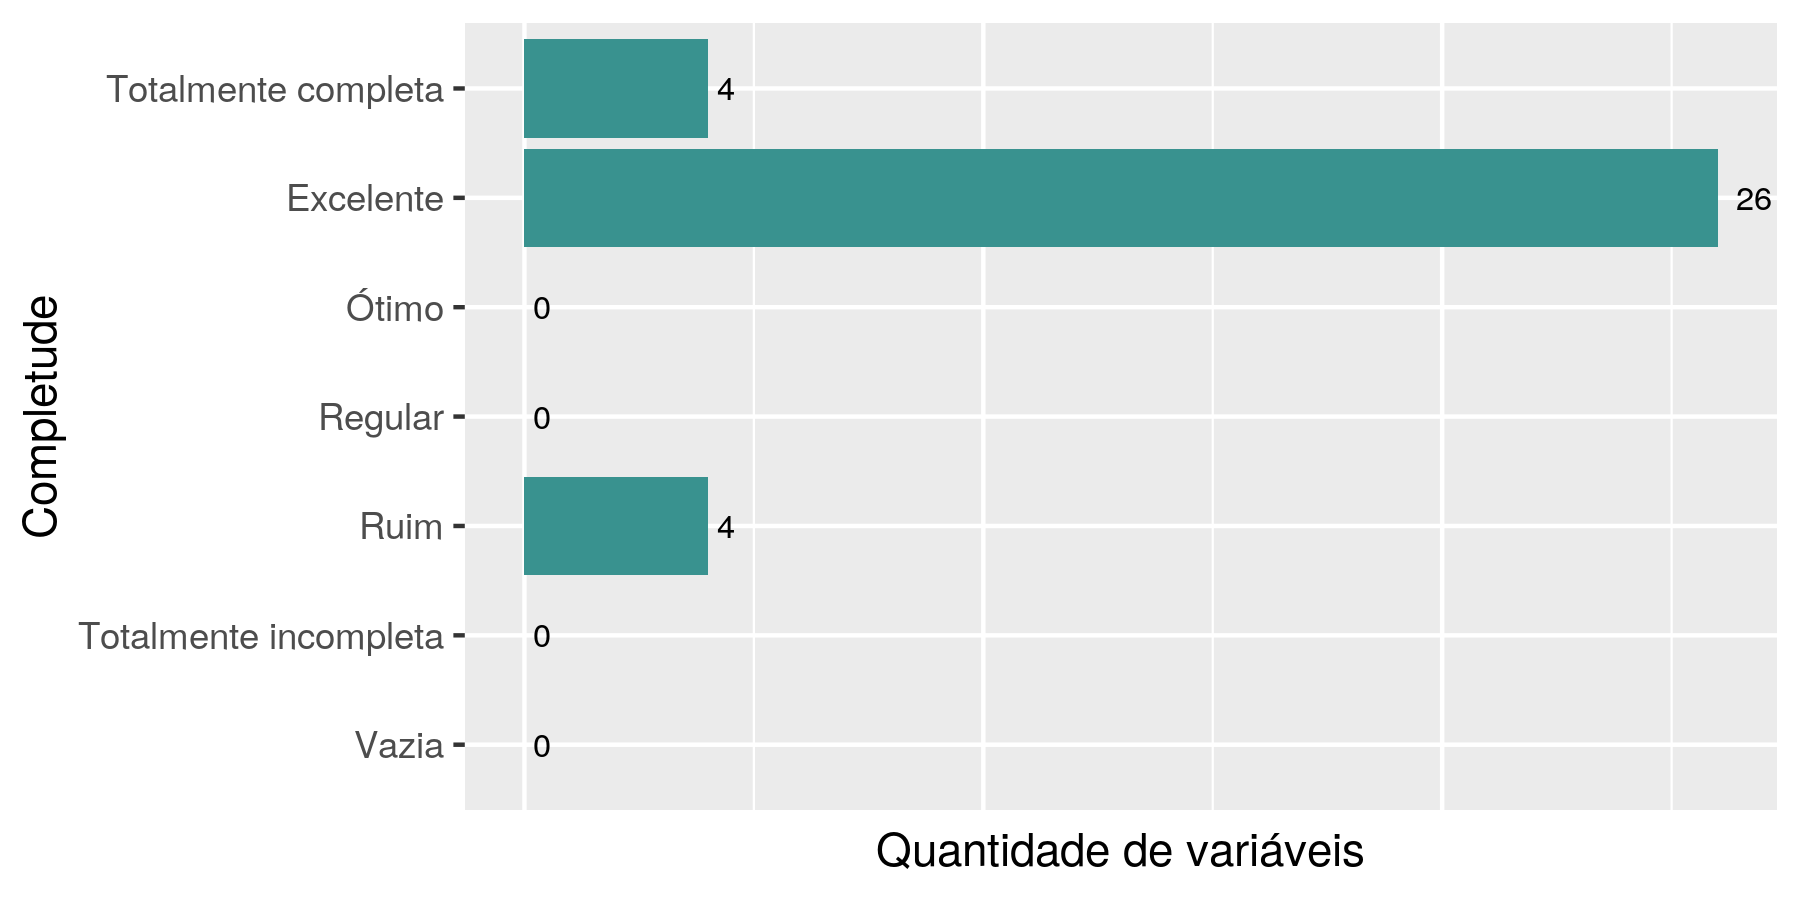
\includegraphics[width=0.8\textwidth,height=\textheight]{imagens/comp.png}
\caption{distribuição dos resultados de completude.}
\end{figure}

\hypertarget{conformidade}{%
\subsection{Conformidade}\label{conformidade}}

Verificou-se se os dados apresentam os padrões descritos no
\protect\hyperlink{dicionuxe1rio-adotado}{dicionário de dados adotado}
como referência a respeito da quantidade de caracteres e valores
válidos.

Acerca das inconformidades identificadas, a tabela a seguir apresenta os
registros mais frequentes, limitado a cinco registros, que encontram-se
nesta situação.

\begingroup\fontsize{10}{12}\selectfont

\begin{longtable}[t]{>{}l>{\raggedright\arraybackslash}p{10cm}}
\caption{\label{tab:unnamed-chunk-13}registros inconformes por variável.}\\
\toprule
Variável & Registros inconformes\\
\midrule
\em{CO\_PACIENTE\_SEXO} & F,\textbackslash{}sM\\
\em{TP\_PACIENTE\_IDENT\_DOC} & 6\\
\bottomrule
\end{longtable}
\endgroup{}

No geral, os resultados de conformidade das variáveis estão distribuídas
pelas categorias definidas em \protect\hyperlink{muxe9todos}{Métodos}
segundo o gráfico a seguir. O resultado percentual por variável está
descrito nos \protect\hyperlink{resultados-numuxe9ricos}{Resultados
numéricos}. O cômputo da média ponderada dos resultados obtidos é de
\textbf{97.12\%}, ou seja, a \textbf{conformidade é excelente}.

\begin{figure}
\centering
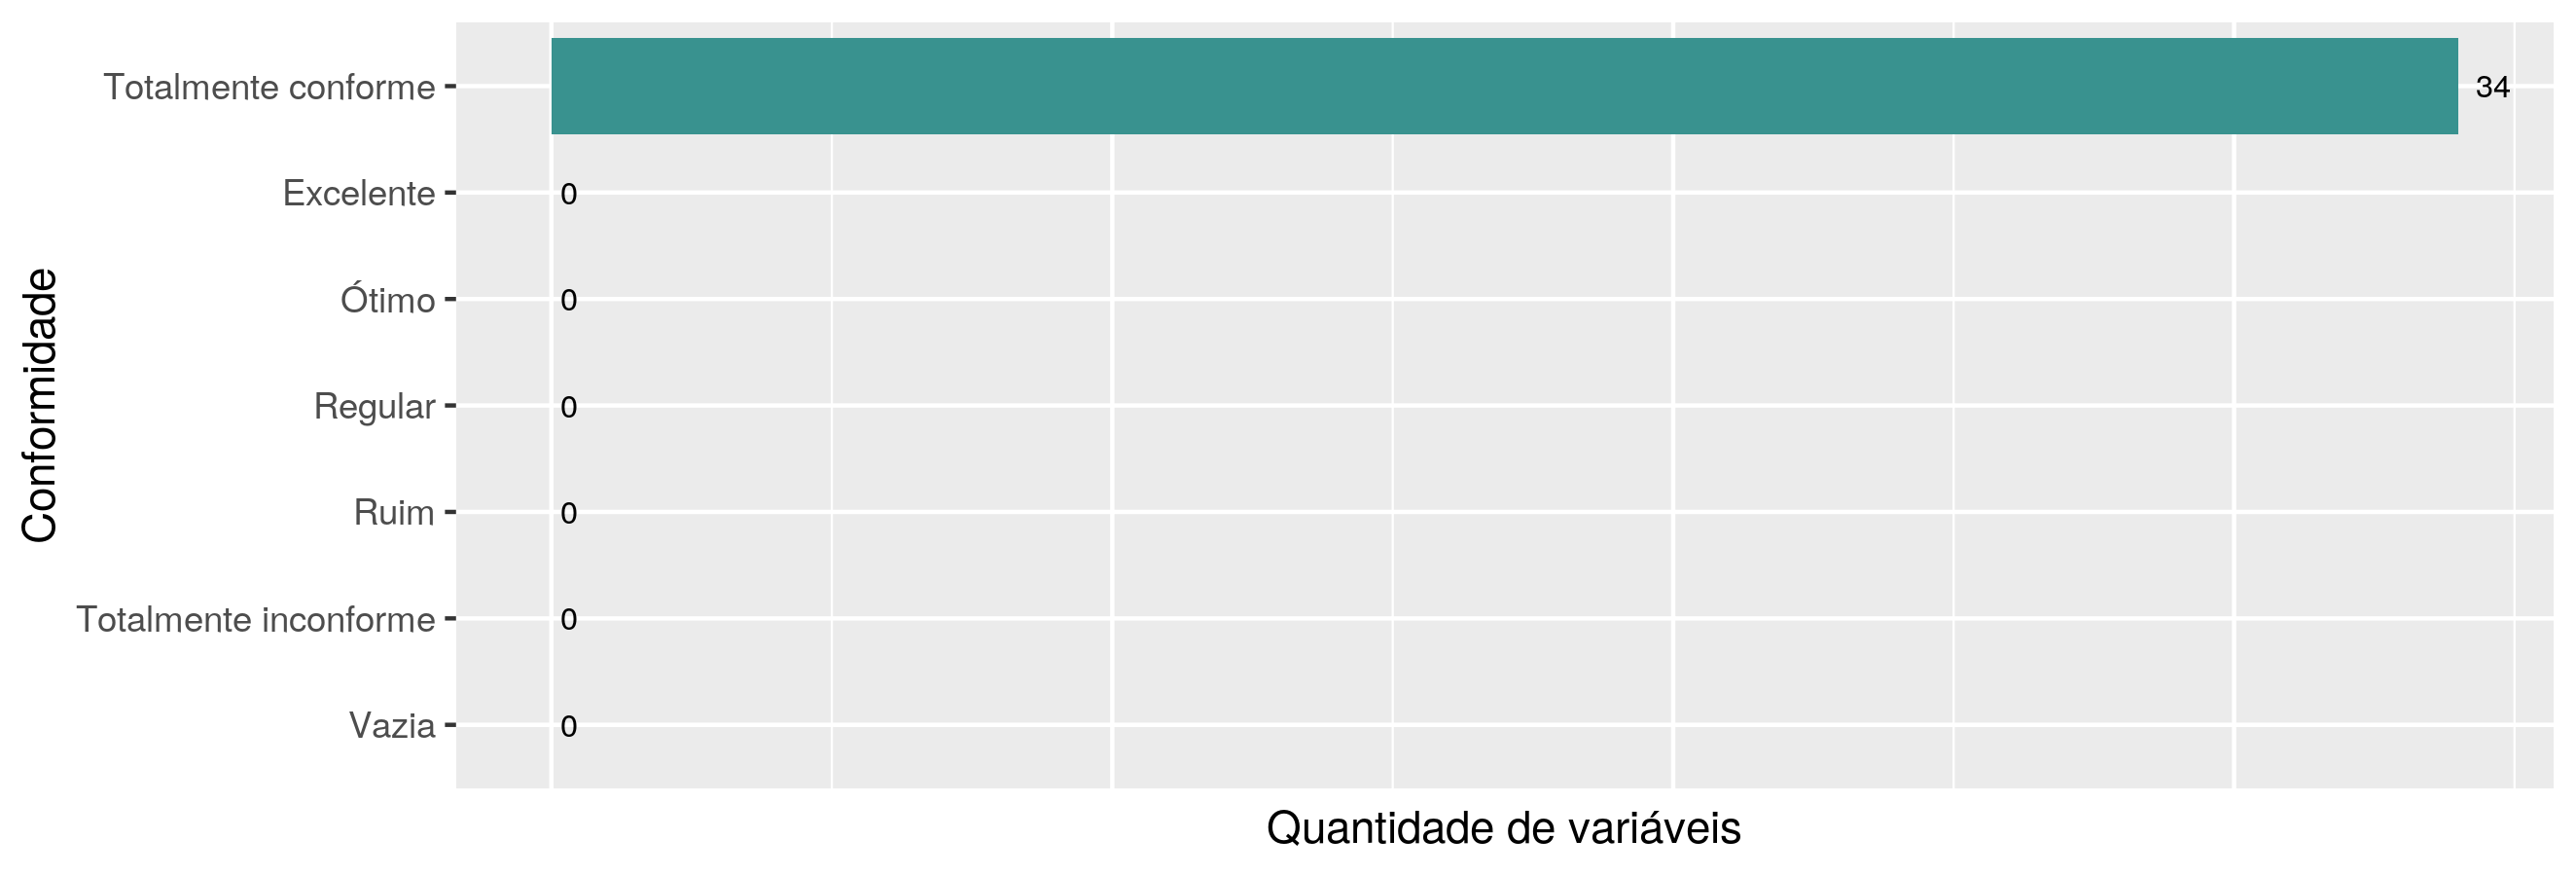
\includegraphics[width=0.8\textwidth,height=\textheight]{imagens/conf.png}
\caption{distribuição dos resultados de conformidade.}
\end{figure}

\hypertarget{acuruxe1cia}{%
\subsection{Acurácia}\label{acuruxe1cia}}

Inicialmente a métrica de acurácia foi aplicada a dois tipos de
registros: datas, ao verificar se o dado configura-se uma data válida e
condizente ao período representado pela base de dados; nomes e códigos
de municípios, ao verificar se estão contidos na tabela de códigos de
municípios e estados do IBGE\footnote{\url{https://www.ibge.gov.br/explica/codigos-dos-municipios.php}}.
Após esta análise de datas e municípios é realizada investigação acerca
do preenchimento das variáveis com o objetivo de detectar a presença de
preenchimentos sem informações relevantes. Em seguida, são verificados
os registros representando informações numéricas, a respeito do sinal
(\emph{e.g.} número de filhos deve ser positivo) e do conjunto ao qual
pertence (\emph{e.g.} número de filhos deve ser um número inteiro).

No que tange propriamente o preenchimento dos registros, buscou-se
identificar valores representando a ausência de informações ou que foram
ignorados, além de sequências finitas do caractere espaço
(\emph{whitespace}) ou sequências finitas do numeral zero para variáveis
não numéricas. Este fato pode representar um problema, visto que estará
de acordo ao tamanho estabelecido pelo dicionário de dados, porém não
estará acurado, não representando informação alguma. Para realizar a
identificação no primeiro caso, utilizou-se o método TF-IDF.

O método TF-IDF\footnote{\url{https://bergvca.github.io/2017/10/14/super-fast-string-matching.html}},
em conjunto aos métodos \emph{N-Grams} e multiplicação de matriz
esparsa, é uma medida estatística que tem o intuito de indicar a
similaridade de uma palavra em relação a outra. TF-IDF é um método para
gerar recursos do texto multiplicando a frequência de um termo em um
documento (\emph{Term Frequency}, ou TF) pela importância (\emph{Inverse
Document Frequency}, ou IDF) do mesmo termo em um corpus inteiro. Este
método é muito útil na classificação e no agrupamento de textos e é
usado para transformar documentos em vetores numéricos, que podem ser
facilmente comparados. Embora os termos no TF-IDF sejam geralmente
palavras, essa condição não é necessária. Como a maioria dos registros
possuem de uma a três palavras, utilizou-se \emph{N-Grams}: sequências
de \emph{N} caracteres contíguos. Para avaliação, calculou-se a
proximidade dos vetores resultantes do método TF-IDF, através da
semelhança cosseno, que pode ser vista como um produto escalar
normalizado.

Após aplicação do método, não identificou-se qualquer registro nessa
situação.

Em relação as várias quantitativas, a tabela a seguir expõe os valores
atípicos detectados\footnote{\url{https://www.rdocumentation.org/packages/grDevices/versions/3.6.2/topics/boxplot.stats}},
isto é, registros numéricos que apresentam grande afastamento em relação
aos demais, dentro do universo de uma única variável, os quais implicam,
tipicamente, em prejuízos a interpretação dos resultados dos testes
estatísticos aplicados.

\begingroup\fontsize{10}{12}\selectfont

\begin{longtable}[t]{>{}l>{\raggedright\arraybackslash}p{10cm}}
\caption{\label{tab:unnamed-chunk-15}valores atípicos para variáveis numéricas.}\\
\toprule
Variável & Valores atípicos\\
\midrule
\endfirsthead
\caption[]{valores atípicos para variáveis numéricas. \textit{(continued)}}\\
\toprule
Variável & Valores atípicos\\
\midrule
\endhead

\endfoot
\bottomrule
\endlastfoot
\em{qt\_diarias} & 12, 13, 14, 15, 16, 17, 18, 19, 20, 21, ..., 277, 278, 304, 305, 306, 307, 310, 336, 337, 338\\
\em{qt\_diarias\_ui} & 1, 2, 3, 4, 5, 6, 7, 8, 9, 10, ..., 69, 70, 72, 74, 80, 91, 93, 99, 100, 101\\
\em{qt\_diarias\_uti} & 1, 2, 3, 4, 5, 6, 7, 8, 9, 10, ..., 101, 102, 105, 106, 107, 114, 115, 117, 127, 134\\
\em{qt\_procedimento} & 4, 5, 6, 7, 8, 9, 10, 11, 12, 13, ..., 598, 600, 604, 621, 629, 646, 677, 794, 980, 996\\
\em{vl\_paciente\_idade} & 116, 118, 119, 122, 123, ..., 116, 118, 119, 122, 123\\
\addlinespace
\em{vl\_valor} & 152.96, 152.97, 152.98, 152.99, 153, 153.01, 153.02, 153.03, 153.04, 153.05, ..., 24530, 25133.04, 26760, 28025.56, 29015.11, 30828.12, 36089.38, 40076.55, 41748, 50000\\*
\end{longtable}
\endgroup{}

Acerca das inacuracidades identificadas, a tabela a seguir apresenta os
registros mais frequentes, limitado a cinco registros, que encontram-se
nesta situação.

\begingroup\fontsize{10}{12}\selectfont

\begin{longtable}[t]{>{}l>{\raggedright\arraybackslash}p{10cm}}
\caption{\label{tab:unnamed-chunk-16}registros inacurados por variável.}\\
\toprule
Variável & Registros inacurados\\
\midrule
\em{CO\_PACIENTE\_SEXO} & I\\
\em{TP\_PACIENTE\_IDENT\_DOC} & IGNORADO\\
\bottomrule
\end{longtable}
\endgroup{}

No geral, os resultados de acurácia das variáveis estão distribuídas
pelas categorias definidas em \protect\hyperlink{muxe9todos}{Métodos}
segundo o gráfico a seguir. O resultado percentual por variável está
descrito nos \protect\hyperlink{resultados-numuxe9ricos}{Resultados
numéricos}. O cômputo da média ponderada dos resultados obtidos é de
\textbf{79.71\%}, ou seja, a \textbf{acurácia é ótimo}.

\begin{figure}
\centering
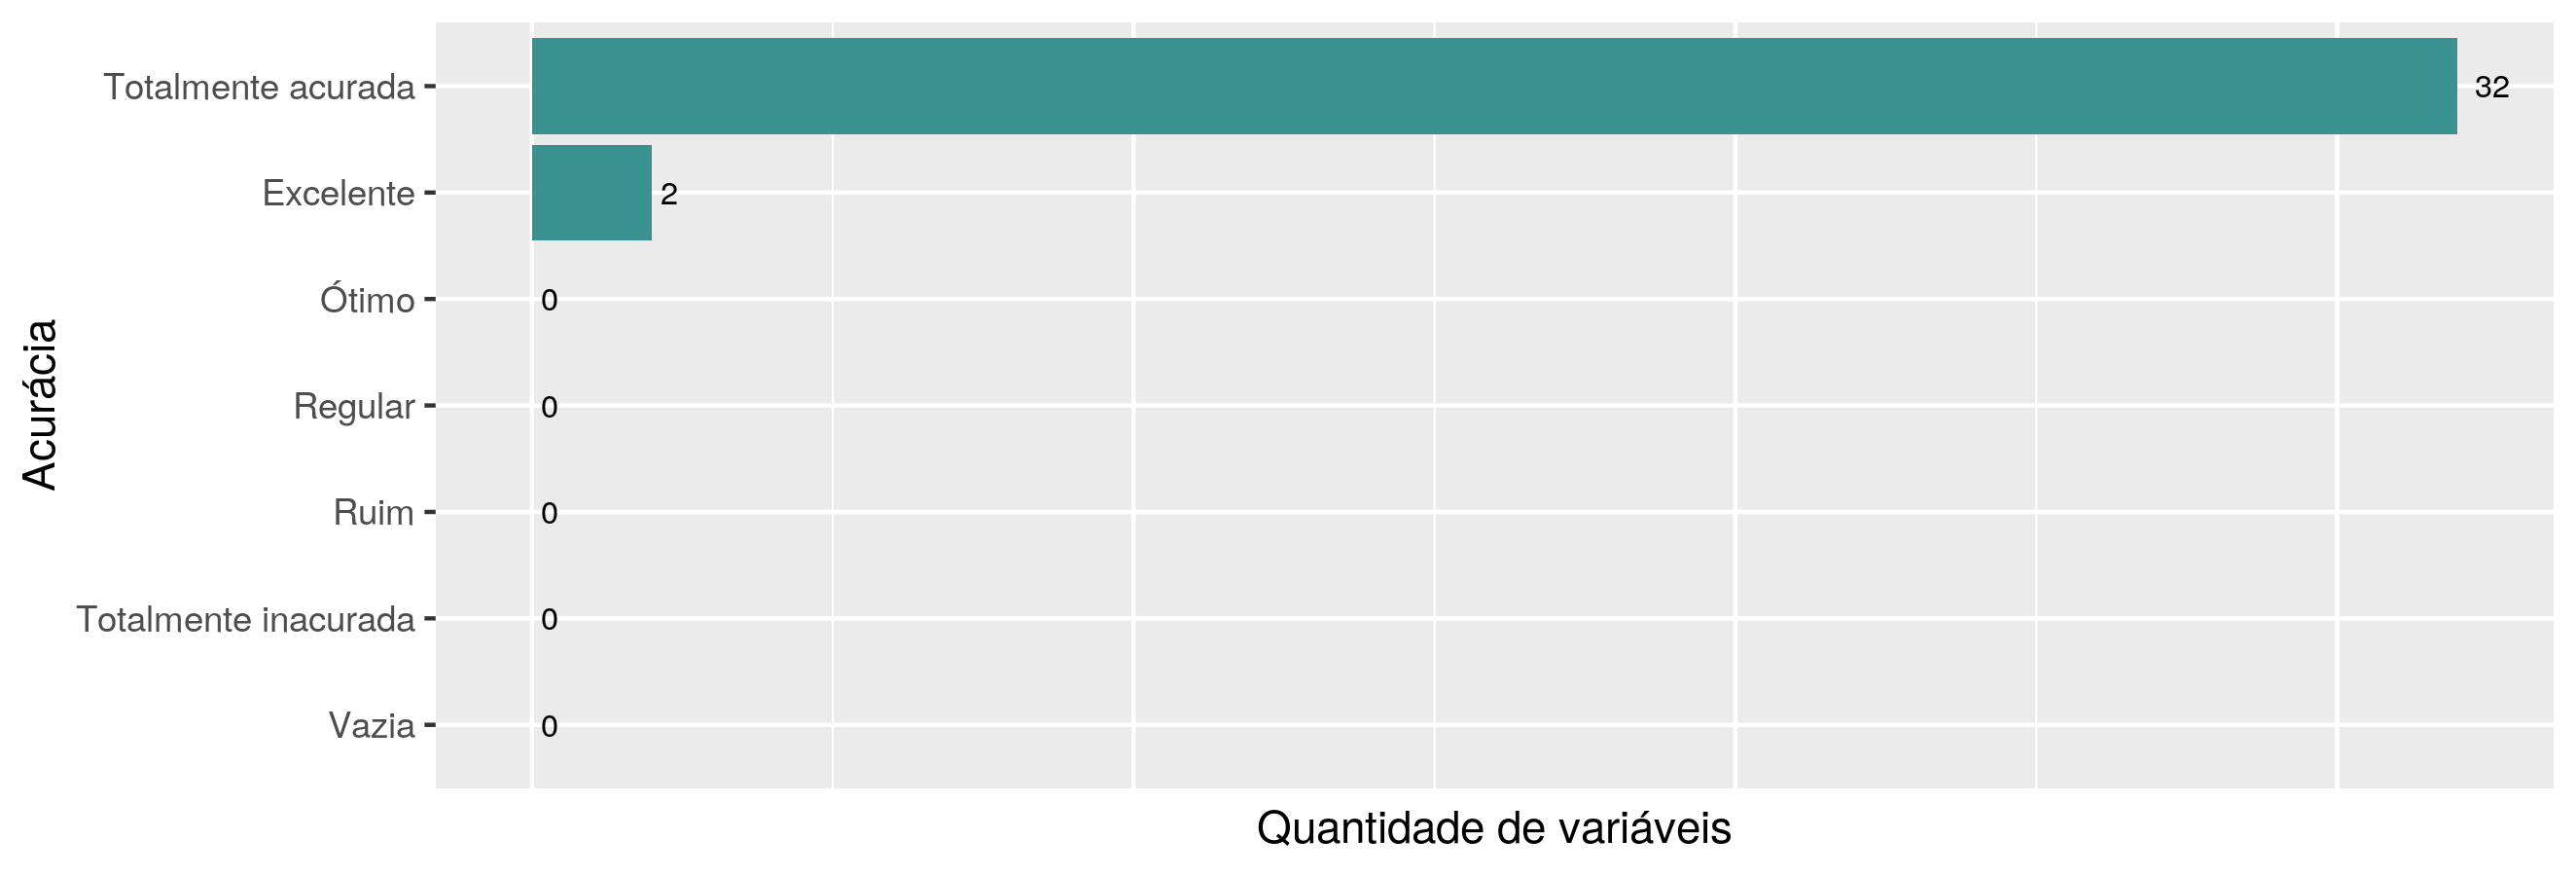
\includegraphics[width=0.8\textwidth,height=\textheight]{imagens/ac.png}
\caption{distribuição dos resultados de acurácia.}
\end{figure}

\hypertarget{consistuxeancia}{%
\subsection{Consistência}\label{consistuxeancia}}

Os resultados apresentados são de testes aplicados a um mesmo registro,
ou seja, mesma linha do conjunto de dados. Estes testes detectam
principalmente problemas na entrada de dados envolvendo condições
específicas de inconsistências. Uma descrição mais detalhada de cada
teste está presente em
\protect\hyperlink{testes-de-inconsistuxeancia}{Testes de
inconsistência}.

\begin{table}[H]

\caption{\label{tab:unnamed-chunk-17}resultados de consistência.}
\centering
\fontsize{10}{12}\selectfont
\begin{tabular}[t]{>{\centering\arraybackslash}p{1cm}>{\raggedright\arraybackslash}p{9cm}>{\centering\arraybackslash}p{3cm}}
\toprule
Teste & Descrição & Falhas [partes por mil]\\
\midrule
\em{T1} & dt\_emissao > dt\_cmp & 3.410\\
\em{T2} & dt\_paciente\_nascimento > dt\_emissao & 0.067\\
\em{T3} & dt\_emissao > dt\_lote\_apres & 0.033\\
\em{T4} & dt\_saida > dt\_cmp & 0.000\\
\em{T5} & dt\_internacao > dt\_cmp & 0.000\\
\addlinespace
\em{T6} & dt\_saida > dt\_lote\_apres & 0.000\\
\em{T7} & dt\_internacao > dt\_lote\_apres & 0.000\\
\em{T8} & dt\_paciente\_nascimento > dt\_saida & 0.000\\
\em{T9} & dt\_internacao > dt\_saida & 0.000\\
\bottomrule
\end{tabular}
\end{table}

A distribuição temporal dos resultados dos testes de consistência é
apresentada no gráfico a seguir

\begin{figure}
\centering
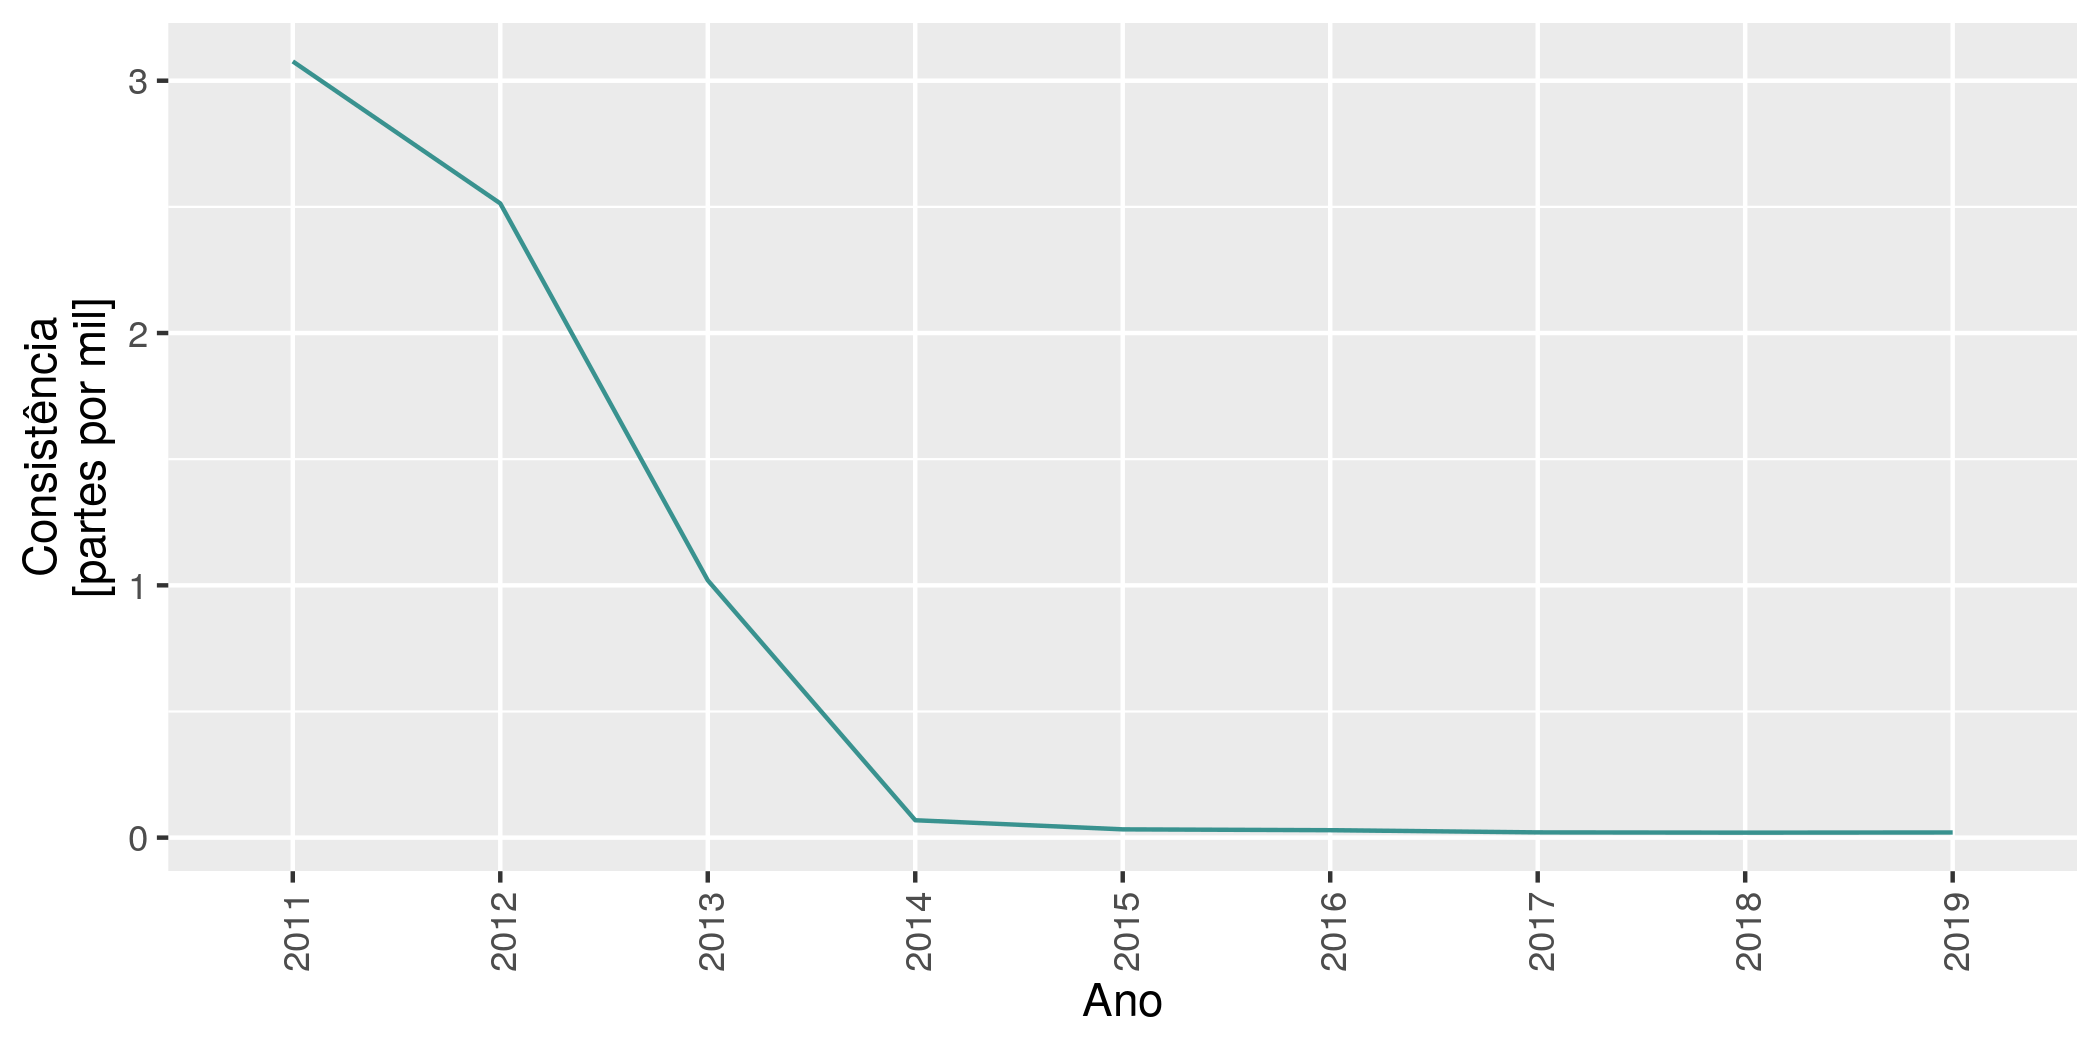
\includegraphics[width=0.8\textwidth,height=\textheight]{imagens/cons-anual.png}
\caption{distribuição temporal da consistência.}
\end{figure}

O resultado de cada teste por ano está descrito em
\protect\hyperlink{testes-de-inconsistuxeancia}{Testes de
inconsistência}. O cômputo da média ponderada dos resultados obtidos é
de \textbf{99.98\%}, ou seja, a \textbf{consistência é excelente}.

\hypertarget{unicidade}{%
\subsection{Unicidade}\label{unicidade}}

\label{sub:unicidade}

Nesta dimensão é calculado o grau de duplicidade dos dados, buscando
diferenças por meio dos identificadores dos pacientes.

São excluídos deste teste os identificadores de pacientes presentes
apenas uma vez na base de dados.

\begin{table}[H]

\caption{\label{tab:unnamed-chunk-19}resultados de unicidade por variável relacionada à identificação do paciente.}
\centering
\fontsize{10}{12}\selectfont
\begin{tabular}[t]{>{}c>{}lc}
\toprule
Teste & Variável & Unicidade [\%]\\
\midrule
\em{T1} & \em{co\_paciente\_nacionalidade} & 99.98\\
\em{T2} & \em{co\_paciente\_sexo} & 99.61\\
\em{T3} & \em{dt\_paciente\_nascimento} & 98.37\\
\em{T4} & \em{co\_raca} & 96.69\\
\em{T5} & \em{raca} & 96.69\\
\bottomrule
\end{tabular}
\end{table}

A distribuição temporal dos resultados dos testes de unicidade é
apresentada no gráfico a seguir.

\begin{figure}
\centering
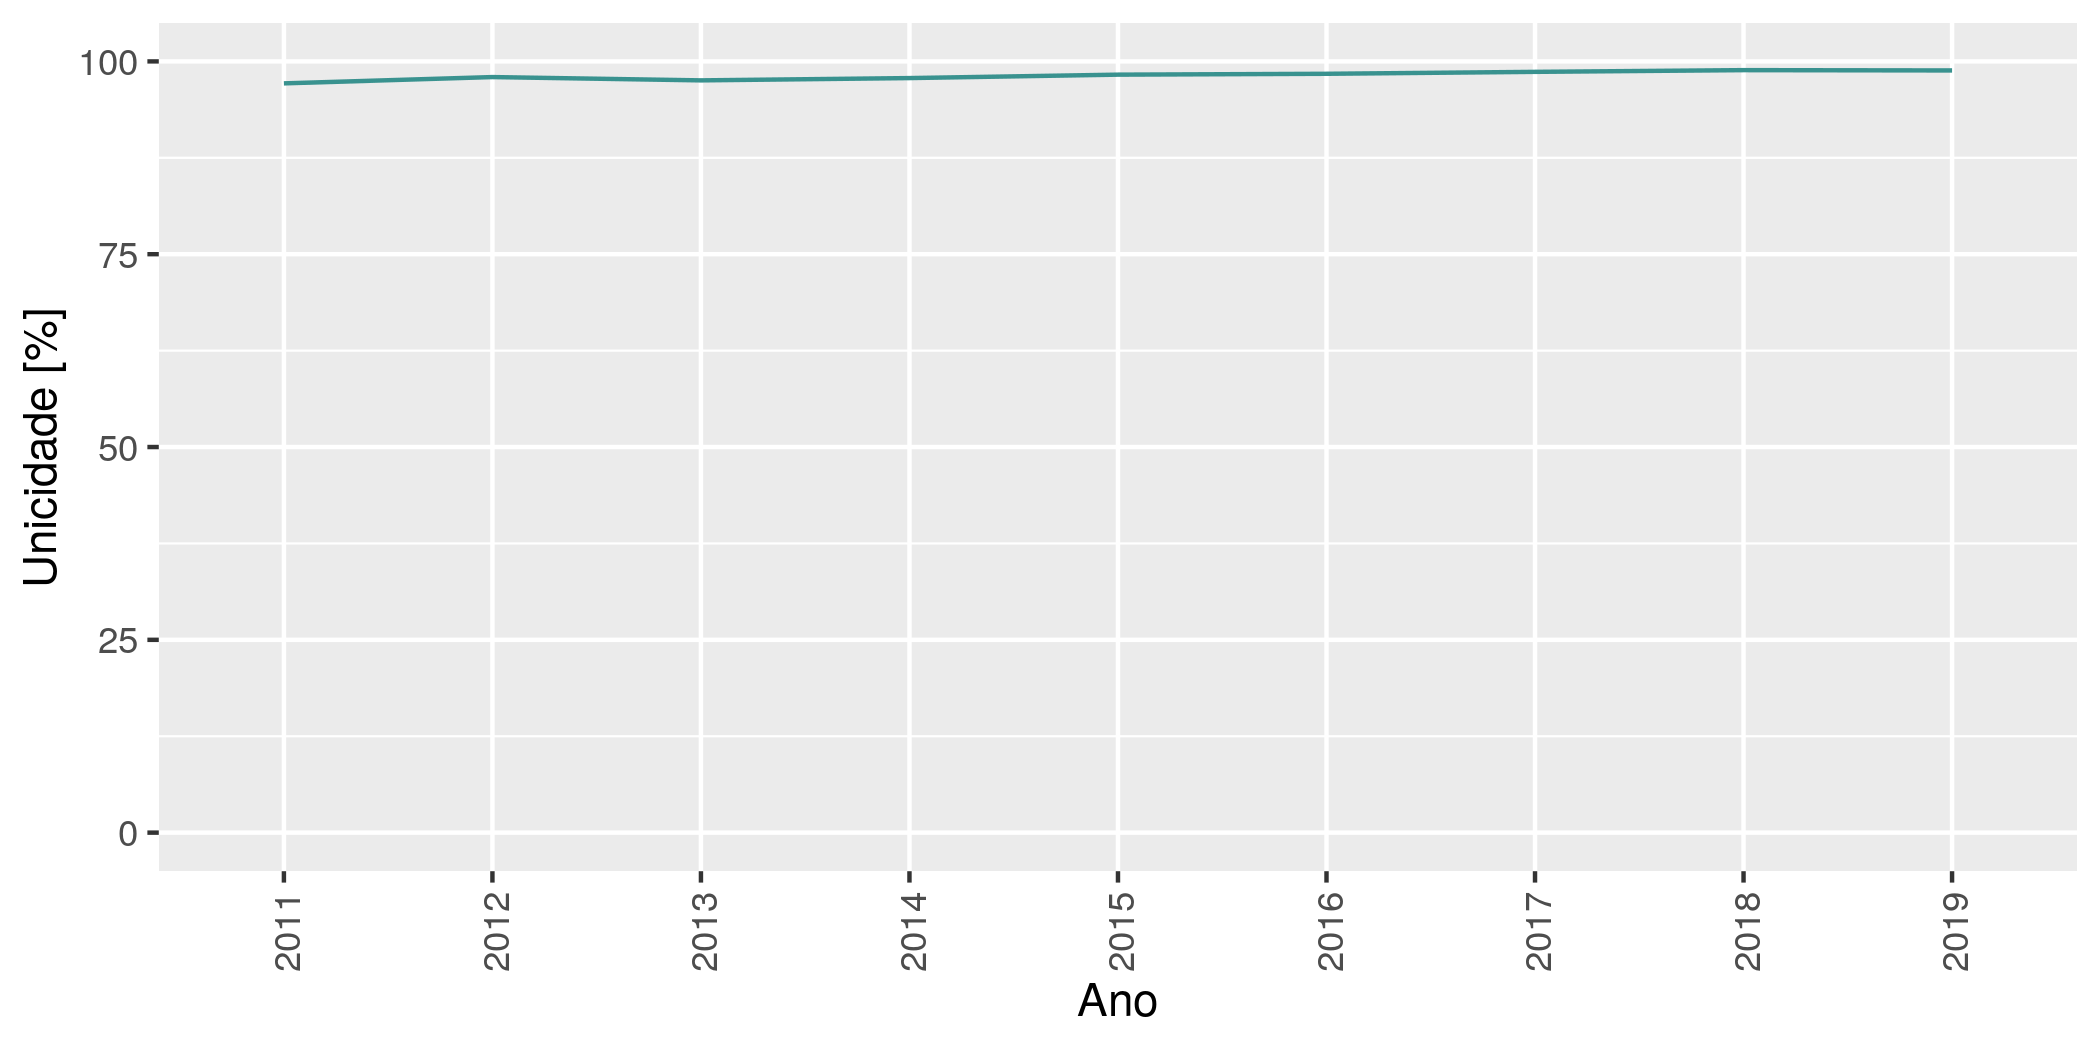
\includegraphics[width=0.8\textwidth,height=\textheight]{imagens/unic-anual.png}
\caption{distribuição temporal da unicidade.}
\end{figure}

O cômputo da média ponderada dos resultados obtidos é de
\textbf{95.07\%}, ou seja, a \textbf{unicidade é excelente}.

\hypertarget{temporalidade}{%
\subsection{Temporalidade}\label{temporalidade}}

Para mensurar esta dimensão é calculada a quantidade de dias entre duas
variáveis representando datas que estejam conformes, acuradas e
consistentes.

\begin{table}[H]

\caption{\label{tab:unnamed-chunk-20}resultados de temporalidade.}
\centering
\fontsize{10}{12}\selectfont
\begin{tabular}[t]{>{}c>{}l>{}lccc}
\toprule
Teste & Variável Inicial & Variável final & Mediana & Min. & Max.\\
\midrule
\em{T1} & \em{dt\_internacao} & \em{dt\_saida} & 4 & 0 & 21000\\
\em{T2} & \em{dt\_emissao} & \em{dt\_lote\_apres} & 52 & 31 & 4300\\
\em{T3} & \em{dt\_emissao} & \em{dt\_cmpt} & 56 & 31 & 4300\\
\bottomrule
\end{tabular}
\end{table}

A distribuição temporal das medianas obtidas pelos testes de
temporalidade é apresentada no gráfico a seguir.

\begin{figure}
\centering
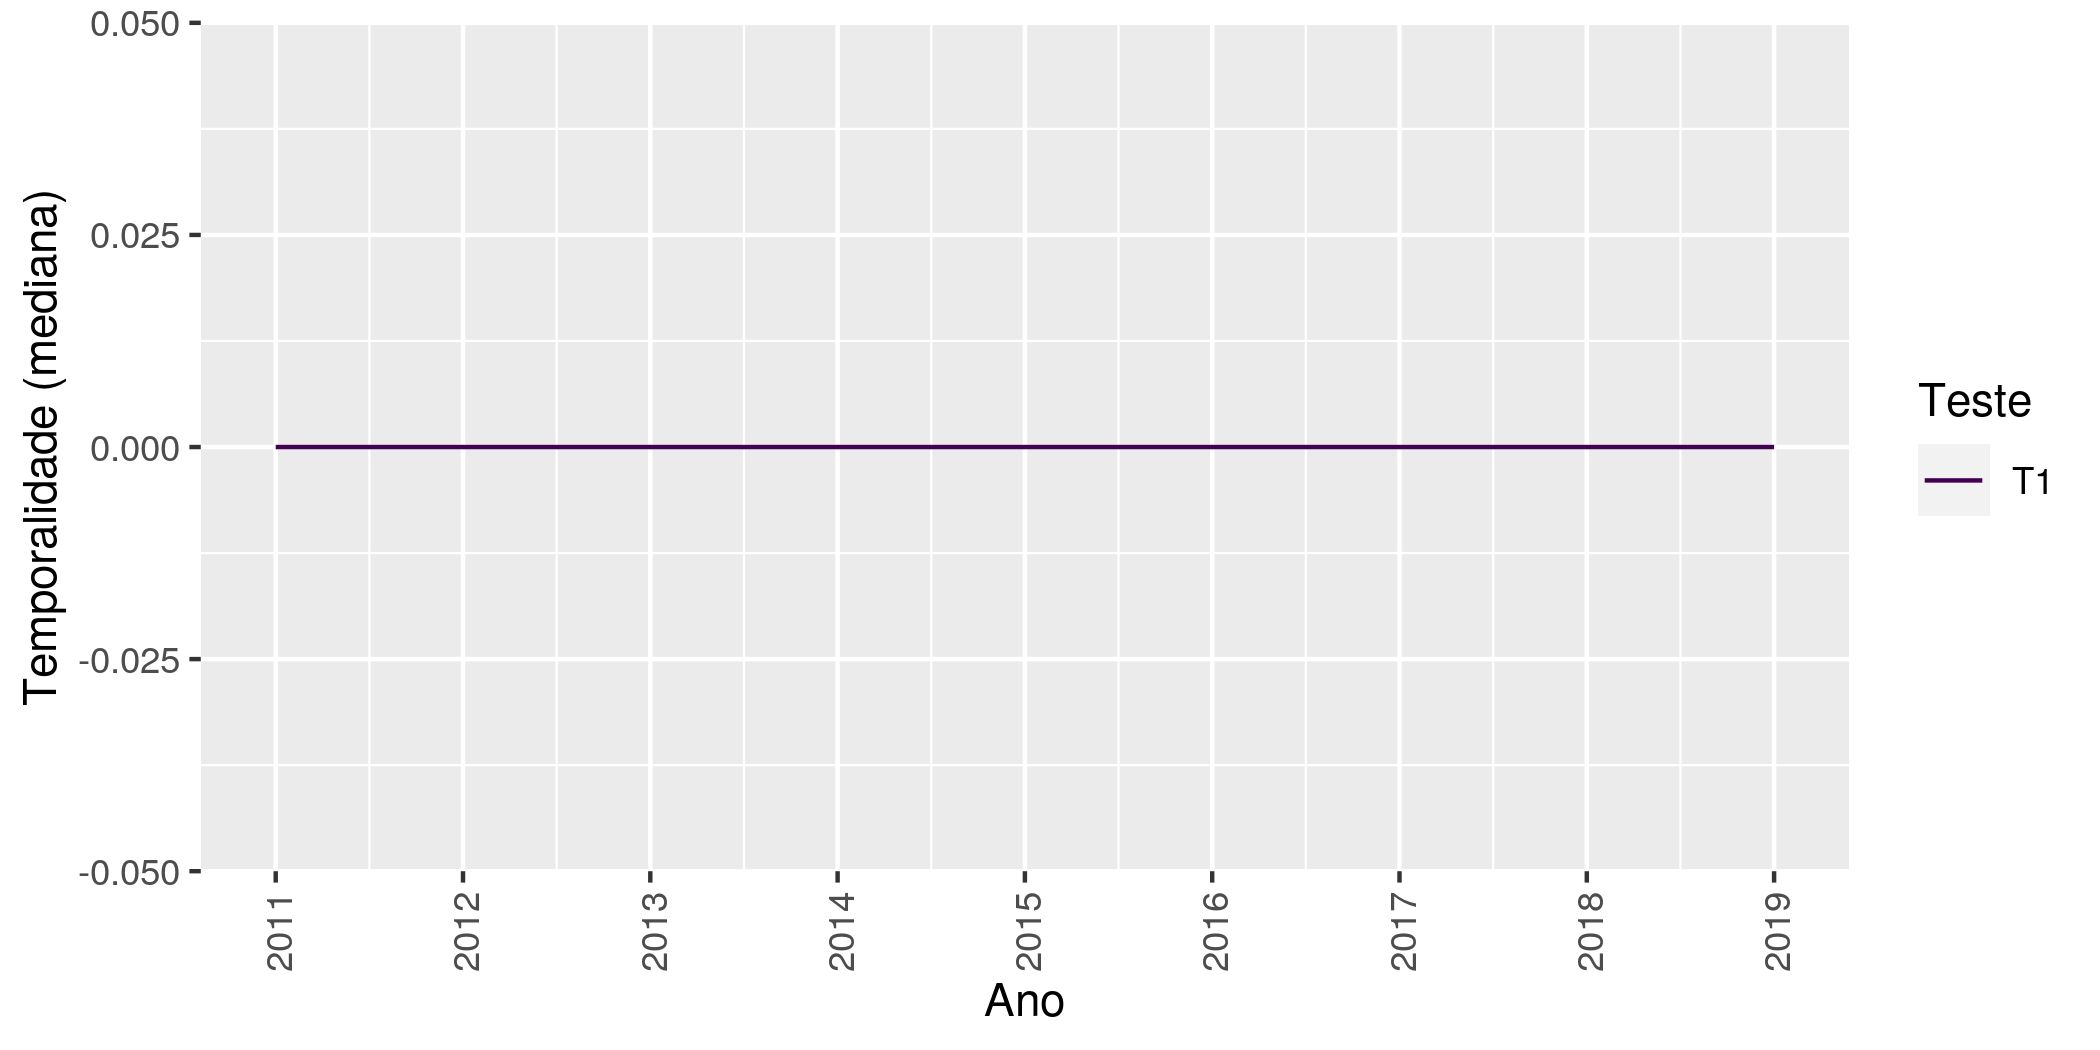
\includegraphics[width=0.8\textwidth,height=\textheight]{imagens/temp-anual.png}
\caption{distribuição temporal da temporalidade.}
\end{figure}

\hypertarget{considerauxe7uxf5es-finais}{%
\section{Considerações finais}\label{considerauxe7uxf5es-finais}}

A avaliação realizada é especialmente oportuna, tendo em vista o cenário
nacional e o atual empenho em fomentar o debate em torno da qualidade
das informações acerca de estabelecimentos de saúde do país.

Assim, a média ponderada dos resultados de Completude é 68.53\%, de
Conformidade é 97.12\%, de Acurácia é 79.71\%, de Consistência é
99.98\%, de Unicidade é 95.07\%. Realizando o produto destes resultados,
obtêm-se \textbf{50.43\%}, caracterizando a \textbf{base de dados como
regular}.

\newpage

\hypertarget{referuxeancias}{%
\section{Referências}\label{referuxeancias}}

\hypertarget{refs}{}
\leavevmode\hypertarget{ref-brasil2019}{}%
Brasil. Ministério da Saúde. Secretaria de Vigilância em Saúde.
Departamento de Análise de Situação em Saúde. 2019. \emph{Saúde Brasil
2019: Uma Análise Da Situação de Saúde Com Enfoque Nas Doenças
Imunopreveníveis E Na Imunização}. Ministério da Saúde.

\leavevmode\hypertarget{ref-merino}{}%
Merino, Jorge, Ismael Caballero, Bibiano Rivas, Manuel Serrano, and
Mario Piattini. 2016. ``A Data Quality in Use Model for Big Data.''
\emph{Future Generation Computer Systems} 63: 123--30.
\url{https://doi.org/https://doi.org/10.1016/j.future.2015.11.024}.

\captionsetup[table]{labelformat=empty}

\newpage

\hypertarget{dicionuxe1rio-adotado}{%
\section*{Dicionário adotado}\label{dicionuxe1rio-adotado}}
\addcontentsline{toc}{section}{Dicionário adotado}

\begingroup\fontsize{10}{12}\selectfont

\begin{longtable}{>{}l>{\raggedright\arraybackslash}p{9cm}>{\centering\arraybackslash}p{2cm}}
\toprule
Variável & Descrição & Tamanho\\
\midrule
\endfirsthead
\multicolumn{3}{@{}l}{\textit{(continued)}}\\
\toprule
Variável & Descrição & Tamanho\\
\midrule
\endhead

\endfoot
\bottomrule
\endlastfoot
\em{co\_car\_internacao} & Caráter da internação. 1: Eletivo, 2: Urgência, 3: Acidente no local trabalho ou a serviço da empresa, 4: Acidente no trajeto para o trabalho, 5: Outros tipo de acidente de trânsito, 6: Outros tipos de lesões e envenenamento por agentes químicos/físicos (baseado de CARATEND.CNV) & [1, 1]\\
\em{co\_cid\_obito} & Código do diagnóstico do óbito. & [1, 4]\\
\em{co\_cid\_principal} & Código do diagnóstico principal. & [1, 4]\\
\em{co\_cid\_secundario} & Código do diagnóstico secundário. & [1, 4]\\
\em{co\_cid\_secundario\_1} & Código do 1º diagnóstico secundário (CID-10). & [1, 4]\\
\addlinespace
\em{co\_cid\_secundario\_2} & Código do 2º diagnóstico secundário (CID-10). & [1, 4]\\
\em{co\_cid\_secundario\_3} & Código do 3º diagnóstico secundário (CID-10). & [1, 4]\\
\em{co\_cid\_secundario\_4} & Código do 4º diagnóstico secundário (CID-10). & [1, 4]\\
\em{co\_cid\_secundario\_5} & Código do 5º diagnóstico secundário (CID-10). & [1, 4]\\
\em{co\_cid\_secundario\_6} & Código do 6º diagnóstico secundário (CID-10). & [1, 4]\\
\addlinespace
\em{co\_cid\_secundario\_7} & Código do 7º diagnóstico secundário (CID-10). & [1, 4]\\
\em{co\_cid\_secundario\_8} & Código do 8º diagnóstico secundário (CID-10). & [1, 4]\\
\em{co\_cid\_secundario\_9} & Código do 9º diagnóstico secundário (CID-10). & [1, 4]\\
\em{co\_cnes} & Código do estabelecimento. & [7, 7]\\
\em{co\_financiamento} & Tipo de financiamento. 0, 9: Não discriminado, 1: Atenção Básica (PAB), 2: Assistência Farmacêutica, 4: Fundo de Ações Estratégicas e Compensações FAEC, 5: Incentivo – MAC, 6: Média e Alta Complexidade (MAC), 7: Vigilância em Saúde (bseado em FINANC.CNV) & [1, 1]\\
\addlinespace
\em{co\_ident} & Identificação do tipo de AIH. NORMAL, DE LONGA PERMANENCIA & [1, 20]\\
\em{co\_modalidade\_internacao} & Modalidade da internação. 02-HOSPITALAR, 03-HOSPITALAR DIA, 04-INTERNACAO DOMICILIAR & [1, 24]\\
\em{co\_mot\_saida} & Motivo da alta do paciente. & [2, 2]\\
\em{co\_oe\_aih} & Código do órgão emissor da AIH. & [10, 10]\\
\em{co\_oe\_gestor} & Código do órgão emissor do gestor (Secretaria). & [10, 10]\\
\addlinespace
\em{co\_paciente\_logr\_cep} & CEP do paciente. & [1, 8]\\
\em{co\_paciente\_logr\_uf} & UF do paciente. & [2, 2]\\
\em{co\_paciente\_nacionalidade} & Código da nacionalidade do paciente. & [1, 3]\\
\em{co\_paciente\_sexo} & Sexo do paciente. M: Masculino, F: Feminino, I: Ignorado & [1, 1]\\
\em{co\_pf\_cbo} & Código no CBO (Código Brasileiro de Ocupações). CBO2002.CNV & [6, 6]\\
\addlinespace
\em{co\_pf\_equipe} &  & [1, 1]\\
\em{co\_proc\_solicitado} & Código do procedimento solicitado. & [9, 9]\\
\em{co\_procedimento\_principal} & Código do procedimento principal realizado no paciente. & [9, 9]\\
\em{co\_raca} & Código da raça/cor do paciente. 0, 9: Sem informação, 1: Branca, 2: Preta, 3: Parda, 4: Amarela, 5: Indígena (baseado em RACACOR.CNV) & [1, 1]\\
\em{co\_seq} &  & [1, 5]\\
\addlinespace
\em{co\_tipo\_faec} &  & [6, 6]\\
\em{cod\_especialidade} & Código da especialidade do leito. 1: Cirúrgico, 2: Obstétricos, 3: Clínico, 4: Crônicos, 5: Psiquiatria, 6: Pneumologia Sanitária (Tisiologia), 7: Pediátricos, 8: Reabilitação, 9: Leito Dia / Cirúrgicos, 10: Leito Dia / Aids, 11: Leito Dia / Fibrose Cística, 12: Leito Dia / Intercorrência Pós-Transplante, 13: Leito Dia / Geriatria, 14: Leito Dia / Saúde Mental, 51: UTI II Adulto COVID 19, 52: UTI II Pediátrica COVID 19, 64: Unidade Intermediária, 65: Unidade Intermediária Neonatal, 74: UTI I, 75: UTI Adulto II, 76: UTI Adulto III, 77: UTI Infantil I, 78: UTI Infantil II, 79: UTI Infantil III, 80: UTI Neonatal I, 81: UTI Neonatal II, 82: UTI Neonatal III, 83: UTI Queimados, 84: Acolhimento Noturno, 85: UTI Coronariana-UCO tipo II, 86: UTI Coronariana-UCO tipo III, 87: Saúde Mental (Clínico), 88: Queimado Adulto (Clínico), 89: Queimado Pediátrico (Clínico), 90: Queimado Adulto (Cirúrgico), 91: Queimado Pediátrico (Cirúrgico), 92: UCI Unidade de Cuidados Intermediarios Neonatal Convencional, 93: UCI Unidade de Cuidados Intermediarios Neonatal Canguru, 94: UCI Unidade de Cuidados Intermediarios Pediatrico, 95: UCI Unidade de Cuidados Intermediarios Adulto, 96: Suporte Ventilatório Pulmonar COVID-19 (baseado de LEITOS.CNV) & [1, 2]\\
\em{cod\_procedimento\_secundario} & Código do procedimento realizado. & [9, 9]\\
\em{complexidade} & Complexidade. 1-ATENCAO BASICA, 2-MEDIA COMPLEXIDADE, 3-ALTA COMPLEXIDADE, 0-NAO SE APLICA (baseado de COMPLEX2.CNV) & [1, 30]\\
\em{desc\_especialidade} &  & [1, 60]\\
\addlinespace
\em{desc\_procedimento\_secundario} &  & [1, 255]\\
\em{ds\_carater} & Conteúdo do campo na tabela. Se chave C-D\_CO\_TAB = 0099 possui o nome das tabelas. URGENCIA, ELETIVO, OUTROS TIPOS DE LESOES E ENVENENAMENTOS POR AGENTES QUIMICOS OU FISICOS, OUTROS TIPOS DE ACIDENTE DE TRANSITO, ACIDENTE NO TRAJETO PARA O TRABALHO (baseado em CARATEND.CNV) & [1, 255]\\
\em{ds\_descricao} & Conteúdo do campo na tabela. Se chave C-D\_CO\_TAB = 0099 possui o nome das tabelas. & [1, 255]\\
\em{ds\_paciente\_logr} & Logradouro do paciente. & [1, 50]\\
\em{ds\_paciente\_logr\_bairro} & Bairro do paciente. & [1, 30]\\
\addlinespace
\em{ds\_paciente\_logr\_compl} & Complemento do endereço do paciente. & [1, 15]\\
\em{dt\_cmpt} & Competência. \%Y\%m & [6, 6]\\
\em{dt\_emissao} & Data da emissão da AIH. \%d/\%m/\%Y & [10, 10]\\
\em{dt\_internacao} & Data da internação do paciente. \%d/\%m/\%Y & [10, 10]\\
\em{dt\_lote\_apres} & Competência de apresentação da AIH ao gestor para processamento. \%m/\%Y & [7, 7]\\
\addlinespace
\em{dt\_paciente\_nascimento} & Data de nascimento do paciente. \%d/\%m/\%Y & [10, 10]\\
\em{dt\_saida} & Data da saída do paciente. \%d/\%m/\%Y & [10, 10]\\
\em{id\_paciente} &  & [1, 12]\\
\em{linha} &  & [1, 3]\\
\em{no\_arq\_remessa} &  & [21, 21]\\
\addlinespace
\em{no\_cbo\_executante} & Descrição da Ocupação da Classificação Brasileira de Ocupações (CBO). & [1, 200]\\
\em{no\_cid\_obito} &  & [1, 100]\\
\em{no\_cid\_principal} &  & [1, 100]\\
\em{no\_cid\_secundario} &  & [1, 100]\\
\em{no\_cid\_secundario\_1} &  & [1, 100]\\
\addlinespace
\em{no\_cid\_secundario\_2} &  & [1, 100]\\
\em{no\_cid\_secundario\_3} &  & [1, 100]\\
\em{no\_cid\_secundario\_4} &  & [1, 100]\\
\em{no\_cid\_secundario\_5} &  & [1, 100]\\
\em{no\_cid\_secundario\_6} &  & [1, 100]\\
\addlinespace
\em{no\_cid\_secundario\_7} &  & [1, 100]\\
\em{no\_cid\_secundario\_8} &  & [1, 100]\\
\em{no\_cid\_secundario\_9} &  & [1, 100]\\
\em{no\_fantasia} &  & [1, 60]\\
\em{no\_municipio} & Campo do nome do município sem acentos. http://www.ibge.gov.br/home/geociencias/areaterritorial/area.shtm & [1, 60]\\
\addlinespace
\em{no\_paciente\_nome} & Nome do paciente. & [1, 70]\\
\em{no\_paciente\_nome\_mae} & Nome da mãe do paciente. & [1, 70]\\
\em{no\_paciente\_nome\_resp} & Nome do responsável pela internação do paciente: parente, amigo etc. & [1, 70]\\
\em{no\_razao\_social} &  & [1, 60]\\
\em{nu\_aih} & Número da AIH. & [13, 13]\\
\addlinespace
\em{nu\_aih\_ant} & Número da AIH anterior (para parto). Quando a paciente é encaminhada para parto, deve ser informado o número da AIH anterior. & [13, 13]\\
\em{nu\_aih\_prox} & Número da próxima AIH (para parto). & [13, 13]\\
\em{nu\_autorizador\_doc} & Número do documento do médico autorizador. & [1, 15]\\
\em{nu\_credito\_doc} & Número do documento. & [1, 15]\\
\em{nu\_dir\_clinico\_doc} & Número do documento do diretor clínico que se responsabiliza pela internação. & [1, 15]\\
\addlinespace
\em{nu\_enfermaria} & Número da enfermaria. & [4, 4]\\
\em{nu\_exec\_doc} & Número do documento. & [1, 15]\\
\em{nu\_gestor\_doc} & Número do documento do gestor (responsável pelo processamento da AIH). & [1, 15]\\
\em{nu\_leito} & Número do leito. & [4, 4]\\
\em{nu\_med\_resp\_doc} & Documento do médico responsável pelo paciente. & [11, 11]\\
\addlinespace
\em{nu\_med\_sol\_doc} & Número do documento do médico que pediu a internação. & [11, 11]\\
\em{nu\_mun\_hosp} & Código IBGE do município do paciente. & [6, 6]\\
\em{nu\_paciente\_logr\_municipio} & Código IBGE do município do paciente. & [6, 6]\\
\em{nu\_paciente\_logr\_numero} & Número do endereço do paciente. & [7, 7]\\
\em{nu\_paciente\_mun\_origem} & Código IBGE do município do paciente. & [6, 6]\\
\addlinespace
\em{nu\_paciente\_numero\_cns} & Número do cartão nacional de saúde (CNS) do paciente. & [15, 15]\\
\em{nu\_paciente\_numero\_doc} & Número do documento do paciente. & [32, 32]\\
\em{nu\_pf\_doc} & Documento de pessoa física. & [15, 15]\\
\em{nu\_pj\_doc} & Documento de pessoa jurídica. & [14, 14]\\
\em{nu\_prontuario} & Número do prontuário do paciente. & [1, 15]\\
\addlinespace
\em{nu\_sisprenatal} & Número da gestante no Pré-Natal. & [12, 12]\\
\em{nu\_versao\_sisaih01} & Versão do SISAIH01. & [1, 4]\\
\em{procedimento\_principal} &  & [1, 250]\\
\em{qt\_diarias} & Total geral de diárias. & [1, 3]\\
\em{qt\_diarias\_ui} & Diárias de unidade intermediária (UI). & [1, 3]\\
\addlinespace
\em{qt\_diarias\_uti} & Diárias de unidade de tratamento intensiva (UTI). & [1, 3]\\
\em{qt\_procedimento} & Quantidade de procedimentos realizados. & [1, 3]\\
\em{raca} & Código da raça/cor do paciente. SEM INFORMACAO, PARDA, BRANCA, PRETA, AMARELA, INDIGENA & [1, 14]\\
\em{sg\_uf} & Sigla da Unidade da Federação. & [2, 2]\\
\em{st\_muda\_proc} & Indicador de mudança de procedimento. 2-NAO, 1-SIM & [1, 5]\\
\addlinespace
\em{st\_situacao} & Situação da AIH. OK, REJEITADA & [1, 9]\\
\em{tp\_ind\_prestador} & Indicador de tipo de prestador. PROPRIO, TERCEIRO & [1, 8]\\
\em{tp\_ind\_rateio} & Indicador de rateio. DIRETO, RATEADO & [1, 7]\\
\em{tp\_ind\_tipo\_valor} & Indicador de tipo de valor. 1, SERVIGO HOSPITALAR: Valor SH , 2, SERVIGO PROFISSIONAL: Valor SP, 3: Valor do complemento federal – SH, 4: Valor do complemento federal – SP, 5: Valor do complemento local – SH, 6: Valor do complemento local – SP (baseado em TP\_VAL.CNV) & [1, 20]\\
\em{tp\_paciente\_ident\_doc} & Identificador do tipo de documento do paciente. IGNORADO, REGISTRO GERAL, CPF, CERTIDAO DE NASCIMENTO, PIS/PASEP & [1, 22]\\
\addlinespace
\em{tp\_paciente\_tipo\_logr} & Tipo de logradouro do paciente: rua, praça, avenida etc. & [1, 3]\\
\em{tp\_pf\_ident} &  & [1, 3]\\
\em{tp\_pj\_ident} & Tipo de identificação. 5-CNES, 3-CNPJ & [1, 6]\\
\em{vl\_paciente\_idade} & Idade do paciente. & [1, 3]\\
\em{vl\_valor} & Valor da parcela. & [1, 8]\\*
\end{longtable}
\endgroup{}

\newpage

\hypertarget{resultados-numuxe9ricos}{%
\section*{Resultados numéricos}\label{resultados-numuxe9ricos}}
\addcontentsline{toc}{section}{Resultados numéricos}

\hypertarget{resultados-gerais}{%
\subsection*{Resultados gerais}\label{resultados-gerais}}
\addcontentsline{toc}{subsection}{Resultados gerais}

\begingroup\fontsize{10}{12}\selectfont

\begin{longtable}{lccc}
\toprule
Variável & Completude [\%] & Conformidade [\%] & Acurácia [\%]\\
\midrule
\endfirsthead
\multicolumn{4}{@{}l}{\textit{(continued)}}\\
\toprule
Variável & Completude [\%] & Conformidade [\%] & Acurácia [\%]\\
\midrule
\endhead

\endfoot
\bottomrule
\endlastfoot
co\_car\_internacao & 100.00 & 100.00 & 100.00\\
co\_cid\_obito & 100.00 & 100.00 & 49.50\\
co\_cid\_principal & 100.00 & 100.00 & 100.00\\
co\_cid\_secundario & 100.00 & 100.00 & 52.45\\
co\_cid\_secundario\_1 & 45.48 & 100.00 & 13.60\\
\addlinespace
co\_cid\_secundario\_2 & 45.48 & 100.00 & 0.10\\
co\_cid\_secundario\_3 & 45.48 & 100.00 & 0.02\\
co\_cid\_secundario\_4 & 45.48 & 100.00 & 0.00\\
co\_cid\_secundario\_5 & 45.48 & 100.00 & 0.00\\
co\_cid\_secundario\_6 & 45.48 & 100.00 & 0.00\\
\addlinespace
co\_cid\_secundario\_7 & 45.48 & 100.00 & 0.00\\
co\_cid\_secundario\_8 & 45.48 & 100.00 & 0.00\\
co\_cid\_secundario\_9 & 45.48 & 100.00 & 0.00\\
co\_cnes & 100.00 & 100.00 & 100.00\\
co\_financiamento & 100.00 & 100.00 & 100.00\\
\addlinespace
co\_ident & 100.00 & 100.00 & 100.00\\
co\_modalidade\_internacao & 100.00 & 100.00 & 100.00\\
co\_mot\_saida & 100.00 & 100.00 & 100.00\\
co\_oe\_aih & 100.00 & 100.00 & 100.00\\
co\_oe\_gestor & 100.00 & 100.00 & 100.00\\
\addlinespace
co\_paciente\_logr\_cep & 0.00 & 0.00 & 0.00\\
co\_paciente\_logr\_uf & 100.00 & 100.00 & 100.00\\
co\_paciente\_nacionalidade & 100.00 & 100.00 & 100.00\\
co\_paciente\_sexo & 100.00 & 0.00 & 0.00\\
co\_pf\_cbo & 100.00 & 20.09 & 100.00\\
\addlinespace
co\_pf\_equipe & 100.00 & 100.00 & 100.00\\
co\_proc\_solicitado & 100.00 & 100.00 & 100.00\\
co\_procedimento\_principal & 100.00 & 100.00 & 100.00\\
co\_raca & 100.00 & 51.66 & 100.00\\
co\_seq & 100.00 & 100.00 & 100.00\\
\addlinespace
co\_tipo\_faec & 100.00 & 100.00 & 0.77\\
cod\_especialidade & 100.00 & 100.00 & 100.00\\
cod\_procedimento\_secundario & 100.00 & 100.00 & 100.00\\
complexidade & 100.00 & 100.00 & 100.00\\
desc\_especialidade & 100.00 & 100.00 & 100.00\\
\addlinespace
desc\_procedimento\_secundario & 100.00 & 100.00 & 100.00\\
ds\_carater & 100.00 & 100.00 & 100.00\\
ds\_descricao & 100.00 & 100.00 & 100.00\\
ds\_paciente\_logr & 0.00 & 0.00 & 0.00\\
ds\_paciente\_logr\_bairro & 100.00 & 100.00 & 73.10\\
\addlinespace
ds\_paciente\_logr\_compl & 0.00 & 0.00 & 0.00\\
dt\_cmpt & 100.00 & 100.00 & 100.00\\
dt\_emissao & 100.00 & 100.00 & 99.69\\
dt\_internacao & 100.00 & 100.00 & 100.00\\
dt\_lote\_apres & 100.00 & 100.00 & 99.12\\
\addlinespace
dt\_paciente\_nascimento & 100.00 & 100.00 & 100.00\\
dt\_saida & 100.00 & 100.00 & 99.69\\
id\_paciente & 90.73 & 100.00 & 100.00\\
linha & 100.00 & 100.00 & 100.00\\
no\_arq\_remessa & 100.00 & 100.00 & 100.00\\
\addlinespace
no\_cbo\_executante & 100.00 & 100.00 & 100.00\\
no\_cid\_obito & 4.03 & 100.00 & 100.00\\
no\_cid\_principal & 100.00 & 100.00 & 100.00\\
no\_cid\_secundario & 6.97 & 100.00 & 100.00\\
no\_cid\_secundario\_1 & 6.18 & 100.00 & 100.00\\
\addlinespace
no\_cid\_secundario\_2 & 0.05 & 100.00 & 100.00\\
no\_cid\_secundario\_3 & 0.01 & 100.00 & 100.00\\
no\_cid\_secundario\_4 & 0.00 & 100.00 & 100.00\\
no\_cid\_secundario\_5 & 0.00 & 100.00 & 100.00\\
no\_cid\_secundario\_6 & 0.00 & 0.00 & 0.00\\
\addlinespace
no\_cid\_secundario\_7 & 0.00 & 0.00 & 0.00\\
no\_cid\_secundario\_8 & 0.00 & 0.00 & 0.00\\
no\_cid\_secundario\_9 & 0.00 & 0.00 & 0.00\\
no\_fantasia & 100.00 & 100.00 & 100.00\\
no\_municipio & 100.00 & 100.00 & 100.00\\
\addlinespace
no\_paciente\_nome & 0.00 & 0.00 & 0.00\\
no\_paciente\_nome\_mae & 0.00 & 0.00 & 0.00\\
no\_paciente\_nome\_resp & 0.00 & 0.00 & 0.00\\
no\_razao\_social & 100.00 & 100.00 & 100.00\\
nu\_aih & 100.00 & 100.00 & 100.00\\
\addlinespace
nu\_aih\_ant & 100.00 & 100.00 & 0.55\\
nu\_aih\_prox & 100.00 & 100.00 & 1.49\\
nu\_autorizador\_doc & 0.00 & 0.00 & 0.00\\
nu\_credito\_doc & 0.00 & 0.00 & 0.00\\
nu\_dir\_clinico\_doc & 0.00 & 0.00 & 0.00\\
\addlinespace
nu\_enfermaria & 100.00 & 100.00 & 60.92\\
nu\_exec\_doc & 0.00 & 0.00 & 0.00\\
nu\_gestor\_doc & 100.00 & 100.00 & 19.91\\
nu\_leito & 100.00 & 100.00 & 60.75\\
nu\_med\_resp\_doc & 0.00 & 0.00 & 0.00\\
\addlinespace
nu\_med\_sol\_doc & 0.00 & 0.00 & 0.00\\
nu\_mun\_hosp & 100.00 & 100.00 & 100.00\\
nu\_paciente\_logr\_municipio & 100.00 & 100.00 & 100.00\\
nu\_paciente\_logr\_numero & 0.00 & 0.00 & 0.00\\
nu\_paciente\_mun\_origem & 0.00 & 0.00 & 0.00\\
\addlinespace
nu\_paciente\_numero\_cns & 0.00 & 0.00 & 0.00\\
nu\_paciente\_numero\_doc & 0.00 & 0.00 & 0.00\\
nu\_pf\_doc & 0.00 & 0.00 & 0.00\\
nu\_pj\_doc & 0.00 & 0.00 & 0.00\\
nu\_prontuario & 100.00 & 100.00 & 100.00\\
\addlinespace
nu\_sisprenatal & 100.00 & 100.00 & 2.95\\
nu\_versao\_sisaih01 & 100.00 & 100.00 & 100.00\\
procedimento\_principal & 100.00 & 100.00 & 100.00\\
qt\_diarias & 100.00 & 100.00 & 100.00\\
qt\_diarias\_ui & 100.00 & 100.00 & 100.00\\
\addlinespace
qt\_diarias\_uti & 100.00 & 100.00 & 100.00\\
qt\_procedimento & 100.00 & 100.00 & 100.00\\
raca & 100.00 & 100.00 & 51.66\\
sg\_uf & 100.00 & 100.00 & 100.00\\
st\_muda\_proc & 100.00 & 100.00 & 100.00\\
\addlinespace
st\_situacao & 100.00 & 100.00 & 87.37\\
tp\_ind\_prestador & 100.00 & 100.00 & 100.00\\
tp\_ind\_rateio & 100.00 & 87.37 & 100.00\\
tp\_ind\_tipo\_valor & 100.00 & 87.37 & 100.00\\
tp\_paciente\_ident\_doc & 100.00 & 99.95 & 40.54\\
\addlinespace
tp\_paciente\_tipo\_logr & 100.00 & 100.00 & 100.00\\
tp\_pf\_ident & 41.73 & 100.00 & 100.00\\
tp\_pj\_ident & 79.34 & 100.00 & 100.00\\
vl\_paciente\_idade & 100.00 & 100.00 & 100.00\\
vl\_valor & 100.00 & 100.00 & 100.00\\*
\end{longtable}
\endgroup{}

\hypertarget{resultados-por-ano}{%
\subsection*{Resultados por ano}\label{resultados-por-ano}}
\addcontentsline{toc}{subsection}{Resultados por ano}

\begingroup\fontsize{10}{12}\selectfont

\begin{longtable}{lccc}
\toprule
Ano & Completude [\%] & Conformidade [\%] & Acurácia [\%]\\
\midrule
\endfirsthead
\multicolumn{4}{@{}l}{\textit{(continued)}}\\
\toprule
Ano & Completude [\%] & Conformidade [\%] & Acurácia [\%]\\
\midrule
\endhead

\endfoot
\bottomrule
\endlastfoot
2008 & 100.00 & 96.65 & 87.29\\
2009 & 100.00 & 96.74 & 87.58\\
2010 & 100.00 & 96.83 & 87.82\\
2011 & 100.00 & 96.71 & 88.18\\
2012 & 100.00 & 96.40 & 88.30\\
\addlinespace
2013 & 100.00 & 96.42 & 88.50\\
2014 & 100.00 & 96.40 & 88.64\\
2015 & 100.00 & 96.65 & 79.90\\
2016 & 100.00 & 96.71 & 78.22\\
2017 & 100.00 & 96.71 & 78.27\\
\addlinespace
2018 & 100.00 & 96.69 & 78.30\\
2019 & 100.00 & 96.71 & 78.03\\*
\end{longtable}
\endgroup{}

\newpage

\hypertarget{testes-de-inconsistuxeancia}{%
\section*{Testes de inconsistência}\label{testes-de-inconsistuxeancia}}
\addcontentsline{toc}{section}{Testes de inconsistência}

\hypertarget{testes-realizados}{%
\subsection*{Testes realizados}\label{testes-realizados}}
\addcontentsline{toc}{subsection}{Testes realizados}

\begin{itemize}
\tightlist
\item
  \textbf{T1}: A data de competência não pode ser menor que a data de
  emissão da AIH
\item
  \textbf{T2}: A data de nascimento do paciente não pode ser maior que a
  data de emissão da AIH
\item
  \textbf{T3}: A data de competência de apresentação da AIH não pode ser
  menor que a data de emissão da AIH
\item
  \textbf{T4}: A data de competência não pode ser menor que a data de
  saída do paciente
\item
  \textbf{T5}: A data de competência não pode ser menor que a data de
  internação do paciente
\item
  \textbf{T6}: A data de competência de apresentação da AIH não pode ser
  menor que a data de saída do paciente
\item
  \textbf{T7}: A data de competência de apresentação da AIH não pode ser
  menor que a data de internação
\item
  \textbf{T8}: A data de nascimento do paciente não pode ser maior que a
  data de saída do paciente
\item
  \textbf{T9}: A data de internação não pode ser maior que a data de
  saída do paciente
\end{itemize}

\hypertarget{resultados-obtidos}{%
\subsection*{Resultados obtidos}\label{resultados-obtidos}}
\addcontentsline{toc}{subsection}{Resultados obtidos}

\begingroup\fontsize{10}{12}\selectfont

\begin{longtable}{>{}cccccccccc}
\toprule
Ano & T1 & T2 & T3 & T4 & T5 & T6 & T7 & T8 & T9\\
\midrule
\endfirsthead
\multicolumn{10}{@{}l}{\textit{(continued)}}\\
\toprule
Ano & T1 & T2 & T3 & T4 & T5 & T6 & T7 & T8 & T9\\
\midrule
\endhead

\endfoot
\bottomrule
\endlastfoot
\em{2008} & 4724 & 161 & 326 & 0 & 0 & 0 & 0 & 0 & 0\\
\em{2009} & 189 & 98 & 0 & 0 & 0 & 0 & 0 & 0 & 0\\
\em{2010} & 429 & 6 & 0 & 0 & 0 & 0 & 0 & 0 & 0\\
\em{2011} & 5793 & 14 & 0 & 0 & 0 & 0 & 0 & 0 & 0\\
\em{2012} & 102 & 53 & 0 & 0 & 0 & 0 & 0 & 0 & 0\\
\addlinespace
\em{2013} & 780 & 97 & 0 & 0 & 0 & 0 & 0 & 0 & 0\\
\em{2014} & 345 & 95 & 0 & 0 & 0 & 0 & 0 & 0 & 0\\
\em{2015} & 351 & 170 & 0 & 0 & 0 & 0 & 0 & 0 & 0\\
\em{2016} & 404 & 146 & 0 & 0 & 0 & 0 & 0 & 0 & 0\\
\em{2017} & 90 & 133 & 0 & 0 & 0 & 0 & 0 & 0 & 0\\
\addlinespace
\em{2018} & 27 & 25 & 0 & 0 & 0 & 0 & 0 & 0 & 0\\
\em{2019} & 60 & 143 & 0 & 0 & 0 & 0 & 0 & 0 & 0\\*
\end{longtable}
\endgroup{}

\end{document}
